\documentclass[11pt]{scaleai-paper}
% Scale AI Research version of the paper (Scale AI x Reflection AI), built with the
% official Scale AI paper class (scaleai-paper.cls). It inputs exactly the same section,
% table, figure and appendix files as main.tex, which remains the anonymous NAACL
% submission. In Overleaf, choose Menu > Main document > main_scale.tex to compile it.

% --- packages the class expects the manuscript to load ---
\usepackage{amsmath,amsfonts,amssymb,amsthm}
\usepackage{booktabs}
\usepackage{tabularx}
\usepackage{tabulary}
\usepackage{multirow}
\usepackage{array}
\usepackage{caption}
\usepackage{subcaption}
\usepackage{float}
\usepackage[square,numbers,sort&compress]{natbib}
\usepackage{xspace}
\usepackage{url}
\usepackage[colorlinks=true,linkcolor=scaleLink,citecolor=scaleLink,urlcolor=scaleLink]{hyperref}
\usepackage[capitalise,nameinlink]{cleveref}
% The template also loads todonotes; it is omitted here because it redefines \todo as a
% margin note, which clashes with the inline \todo notes used in the sections.

% --- this paper's content needs ---
\usepackage{graphicx}
\usepackage{adjustbox}
\usepackage{tikz}
\usetikzlibrary{positioning,arrows.meta,calc}
\usepackage{pifont}

% Shared macros (also defined in main.tex).
\newcommand{\cmark}{\ding{51}}
\newcommand{\xmark}{\ding{55}}
\newcommand{\dyz}[1]{\textcolor{red}{[Daniel: #1]}}
\newcommand{\todo}[1]{\textcolor{blue}{[TODO: #1]}}

% The shared tables and figures scale themselves to \columnwidth for the two-column ACL
% layout. In this one-column layout that would enlarge them, so here \resizebox only
% shrinks content that is wider than the target width.
\renewcommand{\resizebox}[3]{\adjustbox{max width=#1}{#3}}

% --- front matter (Scale AI template) ---
\papertype{Scale AI Research}
\scaleailogopath{assets/scale-logo-horizontal.png}
\partnerlogopath{assets/reflection-logo.pdf}
\partnerlogoheight{0.2in}
\contact{\texttt{yue.zhang@scale.com}}

\title{SWE-Bench Pro V2: A Cleaner, Harder-to-Game Coding Benchmark}

% AUTHORS: same list as main.tex. Add affiliation indices once confirmed,
% e.g. \author[1]{...} for Scale AI and \author[2]{...} for Reflection AI.
\author{Soham Dan}
\author{Jeff Da}
\author{Sanyam Bhutani}
\author{Miguel Romero}
\author{\placeholder{additional authors TBD}}
\author{Ying Liu}
\author{Daniel Yue Zhang}
\affil[1]{Scale AI}
\affil[2]{Reflection AI}

\begin{document}
\maketitle

\begin{abstract}
SWE-Bench Pro is a widely used benchmark of long-horizon software engineering tasks for evaluating coding agents. As agents have become more capable, they have begun to surface task issues that earlier agents rarely reached, and they interact with the evaluation environment in ways the original harness did not anticipate. We present SWE-Bench Pro V2, a revised release of the public split designed to keep the benchmark accurate as capabilities advance. Two agentic audits, followed by expert adjudication and blind re-implementation, identify issues in 20\% of the original tasks, such as specifications that do not fully describe what the hidden tests check and verifiers that reject correct solutions; these tasks are revised or retired. V2 also adopts a hardened evaluation protocol that restricts network access to the model endpoint and re-grades every patch in a clean container, so that agents cannot retrieve upstream fixes or receive credit for changes outside their patch. On the 642 V2 tasks, frontier agents resolve up to 99.4\% while other systems remain clearly separated, and a new \nHard{}-task Hard split spreads systems from 25.5\% to 98.0\%. On a never-public set, the same revisions raise pass rates on revised tasks by 16.4 points and leave the remaining tasks nearly unchanged. We release the benchmark, the protocol and per-task grades, and we summarize lessons for maintaining agent benchmarks over time.
% TODO: add one sentence on the harness comparison (Section 4.6) once finalized.
% Camera-ready: state that V2 is released by the maintainers of the original SWE-Bench Pro (omitted for double-blind review).
\end{abstract}

\section{Introduction}

Benchmarks built from real GitHub issues have become a standard to compare coding agents. SWE-bench \citep{jimenez2024swebench} asks an agent to resolve an issue in a real repository and grades the resulting patch with the tests of the original fix. After frontier systems saturated its human-screened subset, SWE-bench Verified \citep{openai2024verified}, and contamination of its older issues became difficult to rule out, it was no longer used to measure frontier capability \citep{openai2026swebenchverified}. SWE-Bench Pro \citep{deng2025swebenchpro} was designed as its successor. Its public split contains 731 tasks from 11 actively maintained repositories in Python, Go and JavaScript/TypeScript. Reference solutions often span several files, and each task pairs a human-written specification (problem statement, requirements and interface) with hidden tests. SWE-Bench Pro scores are widely reported in model releases and leaderboards, and practitioners use them to select models and agent scaffolds, so keeping the benchmark accurate over time is crucial.

As agents improve, a growing share of their remaining failures traces back to issues in the tasks \citep{nadgir2026life}. We reviewed all 731 public tasks and found two classes of issues. \emph{Data defects} make a task's grade disagree with the correctness of the solution: tests that check behaviour the instruction never states, instructions that contradict or leak the tests, weak tests, and verifier or environment defects (Table~\ref{tab:repairs-discards}); repairing or retiring them touched 480 tasks (66\%). \emph{Evaluation exploits} let an agent pass by cheating, without solving the task.


We address both classes of issues and release SWE-Bench Pro V2. Two agentic audits flag 200 of the 731 tasks, 23 expert software engineers adjudicate every flag, and the verifiers are hardened for all tasks (Figure~\ref{fig:pipeline}). The release has 642 tasks, 391 repaired and 89 discarded.

On V2 the Claude system resolves 99\% of the tasks whereas Gemini~3.8 Flash resolves 94.9\% and Inkling 89.9\% (Figure~\ref{fig:spread}). The full set still separates systems below the frontier, and a 51-task Hard split spreads systems from 52.9\% to 98.0\%. 

Our contributions are:
\begin{itemize}\setlength\itemsep{0pt}
\item \textbf{SWE-Bench Pro V2}: 642 tasks and a 51-task Hard split, after several rounds of automatic and expert repair: 23 engineers adjudicate every agentic audit flag (404 hours), validated each repair by blind re-implementation, and hardened and gated every verifier (\S\ref{sec:method}).

\item \textbf{A repair pipeline and defect taxonomy} for issue-based coding benchmarks, with agentic audits as triage, engineer adjudication, blind re-implementation and verifier hardening (\S\ref{sec:audits}--\ref{sec:verifier}).

\item \textbf{Evidence from operating the benchmark}: the exploits that in-sandbox grading admits and the locked protocol rejects (\S\ref{sec:protocol-results}), a study showing the agent harness changes cost but not accuracy for open-weight models (\S\ref{sec:harness}), and why a benchmark near saturation for frontier models remains useful (\S\ref{sec:discussion}).

\end{itemize}

%We address both classes of issues and release the result as SWE-Bench Pro V2 (\S\ref{sec:method}). The data pipeline has four stages. (1)~The two agentic audits flag 200 of the 731 tasks. (2)~23 software engineers adjudicate every flag against the task artifacts, spending 1{,}897 hours in total. They edit an instruction only where a flag is confirmed, never modify a hidden test to match an instruction, and discard tasks whose defect lies in the tests, verifier or image. (3)~In a quality-control stage, a second engineer who has seen neither the original task nor the reference patch implements each edited instruction, and the repair is accepted only if this implementation passes the hidden tests. High-priority flags additionally receive a second independent review. (4)~We harden the shared verifiers and require, before release, that the reference patch passes and the empty patch fails on every task. The release contains 642 tasks (531 never flagged, 66 repaired and 45 flagged but kept), and 89 tasks were discarded. For the evaluation, a locked protocol allows the agent to reach only the model endpoint, verifies this restriction before every run, and grades each patch in a fresh container. \jeff{Can we make figure 2 match this paragraph's 4 stages?}

%On V2, the strongest systems solve almost every task (Figure~\ref{fig:spread}). The three Claude systems resolve 99.1--99.4\% and are statistically tied, so the full set no longer distinguishes frontier systems, although it still distinguishes the others. Gemini~3.8 Flash resolves 94.9\% and Inkling 89.9\%. Because every task is solvable and correctly graded, these gaps can be attributed to the systems; our audit attributes only 3 of Gemini's 33 failures to residual task defects. To recover spread at the top, we release a Hard split of 51 tasks on which systems range from 25.5\% to 98.0\%. The split also separates two systems that are tied on the remaining tasks. The full set remains useful for evaluating smaller and open-weight systems, whose differences were previously confounded by a 20\% defect rate. Finally, on a never-public set, correcting instructions raises the pass rate on the corrected tasks by 16.4 points and changes the other tasks by less than one point. \jeff{I think this paragraph can also be shorter or doesn't need so much detail?}

% Our contributions are as follows:
% \begin{itemize}\setlength\itemsep{0pt}
% \item \textbf{A defect taxonomy and repair pipeline} for issue-based coding benchmarks that combines two agentic audits with engineer adjudication and blind re-implementation, applied to every public SWE-Bench Pro task (\S\ref{sec:audits}--\ref{sec:review}).
% \item \textbf{SWE-Bench Pro V2}, 642 repaired tasks with hardened verifiers, and a 51-task Hard split that separates frontier systems (\S\ref{sec:verifier}, \S\ref{sec:hard}) \jeff{this should be the main contribution at the top? a hardened benchmark with 1.5k+ expert hours of annotation, multiple rounds of review, and acting as a new standard.}
% \item \textbf{A locked evaluation protocol} that restricts the network to the model endpoint and re-grades every patch in a fresh container. Under this protocol, no run retrieved external content, and re-grading rejected every dependency forged outside the patch (\S\ref{sec:protocol}, \S\ref{sec:protocol-results}) \jeff{we might not need to mention this because it's a bit of an industry standard}.
% \item \textbf{Evidence and lessons from operating the benchmark}, including a controlled study on a never-public set showing that data repairs change scores on the repaired tasks, an analysis of the benchmark's usefulness near saturation, a study of how the agent harness changes the behaviour of strong open-weight models, and practical lessons for benchmark maintainers (\S\ref{sec:private}, \S\ref{sec:harness}, \S\ref{sec:discussion}).
% \end{itemize}
%We release the tasks, the Hard split, the harness configuration and the per-task grades of every run.\todo{Anonymized link.}

\begin{figure}[t]
\centering\footnotesize
\resizebox{\columnwidth}{!}{%
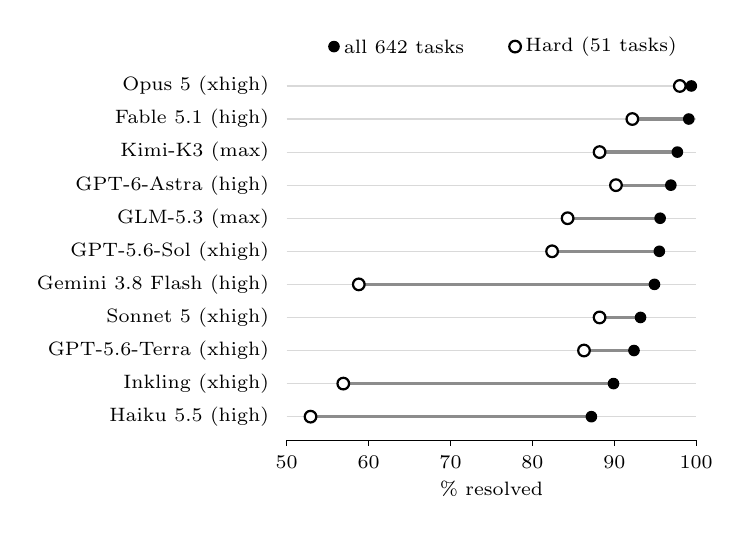
\begin{tikzpicture}
\node[anchor=east,font=\scriptsize] at (-0.1,0.00) {Opus 5 (xhigh)};
\draw[gray!30] (0,0.00) -- (5.2,0.00);
\draw[line width=1.2pt,black!45] (4.992,0.00) -- (5.138,0.00);
\fill[black] (5.138,0.00) circle (2.1pt);
\draw[black,fill=white,line width=0.8pt] (4.992,0.00) circle (2.1pt);
\node[anchor=east,font=\scriptsize] at (-0.1,-0.42) {Fable 5.1 (high)};
\draw[gray!30] (0,-0.42) -- (5.2,-0.42);
\draw[line width=1.2pt,black!45] (4.389,-0.42) -- (5.106,-0.42);
\fill[black] (5.106,-0.42) circle (2.1pt);
\draw[black,fill=white,line width=0.8pt] (4.389,-0.42) circle (2.1pt);
\node[anchor=east,font=\scriptsize] at (-0.1,-0.84) {Kimi-K3 (max)};
\draw[gray!30] (0,-0.84) -- (5.2,-0.84);
\draw[line width=1.2pt,black!45] (3.973,-0.84) -- (4.961,-0.84);
\fill[black] (4.961,-0.84) circle (2.1pt);
\draw[black,fill=white,line width=0.8pt] (3.973,-0.84) circle (2.1pt);
\node[anchor=east,font=\scriptsize] at (-0.1,-1.26) {GPT-6-Astra (high)};
\draw[gray!30] (0,-1.26) -- (5.2,-1.26);
\draw[line width=1.2pt,black!45] (4.181,-1.26) -- (4.878,-1.26);
\fill[black] (4.878,-1.26) circle (2.1pt);
\draw[black,fill=white,line width=0.8pt] (4.181,-1.26) circle (2.1pt);
\node[anchor=east,font=\scriptsize] at (-0.1,-1.68) {GLM-5.3 (max)};
\draw[gray!30] (0,-1.68) -- (5.2,-1.68);
\draw[line width=1.2pt,black!45] (3.567,-1.68) -- (4.742,-1.68);
\fill[black] (4.742,-1.68) circle (2.1pt);
\draw[black,fill=white,line width=0.8pt] (3.567,-1.68) circle (2.1pt);
\node[anchor=east,font=\scriptsize] at (-0.1,-2.10) {GPT-5.6-Sol (xhigh)};
\draw[gray!30] (0,-2.10) -- (5.2,-2.10);
\draw[line width=1.2pt,black!45] (3.370,-2.10) -- (4.732,-2.10);
\fill[black] (4.732,-2.10) circle (2.1pt);
\draw[black,fill=white,line width=0.8pt] (3.370,-2.10) circle (2.1pt);
\node[anchor=east,font=\scriptsize] at (-0.1,-2.52) {Gemini 3.8 Flash (high)};
\draw[gray!30] (0,-2.52) -- (5.2,-2.52);
\draw[line width=1.2pt,black!45] (0.915,-2.52) -- (4.670,-2.52);
\fill[black] (4.670,-2.52) circle (2.1pt);
\draw[black,fill=white,line width=0.8pt] (0.915,-2.52) circle (2.1pt);
\node[anchor=east,font=\scriptsize] at (-0.1,-2.94) {Sonnet 5 (xhigh)};
\draw[gray!30] (0,-2.94) -- (5.2,-2.94);
\draw[line width=1.2pt,black!45] (3.973,-2.94) -- (4.493,-2.94);
\fill[black] (4.493,-2.94) circle (2.1pt);
\draw[black,fill=white,line width=0.8pt] (3.973,-2.94) circle (2.1pt);
\node[anchor=east,font=\scriptsize] at (-0.1,-3.36) {GPT-5.6-Terra (xhigh)};
\draw[gray!30] (0,-3.36) -- (5.2,-3.36);
\draw[line width=1.2pt,black!45] (3.775,-3.36) -- (4.410,-3.36);
\fill[black] (4.410,-3.36) circle (2.1pt);
\draw[black,fill=white,line width=0.8pt] (3.775,-3.36) circle (2.1pt);
\node[anchor=east,font=\scriptsize] at (-0.1,-3.78) {Inkling (xhigh)};
\draw[gray!30] (0,-3.78) -- (5.2,-3.78);
\draw[line width=1.2pt,black!45] (0.718,-3.78) -- (4.150,-3.78);
\fill[black] (4.150,-3.78) circle (2.1pt);
\draw[black,fill=white,line width=0.8pt] (0.718,-3.78) circle (2.1pt);
\node[anchor=east,font=\scriptsize] at (-0.1,-4.20) {Haiku 5.5 (high)};
\draw[gray!30] (0,-4.20) -- (5.2,-4.20);
\draw[line width=1.2pt,black!45] (0.302,-4.20) -- (3.869,-4.20);
\fill[black] (3.869,-4.20) circle (2.1pt);
\draw[black,fill=white,line width=0.8pt] (0.302,-4.20) circle (2.1pt);
\draw (0,-4.50) -- (5.2,-4.50);
\draw (0.000,-4.50) -- (0.000,-4.57) node[below,font=\scriptsize] {50};
\draw (1.040,-4.50) -- (1.040,-4.57) node[below,font=\scriptsize] {60};
\draw (2.080,-4.50) -- (2.080,-4.57) node[below,font=\scriptsize] {70};
\draw (3.120,-4.50) -- (3.120,-4.57) node[below,font=\scriptsize] {80};
\draw (4.160,-4.50) -- (4.160,-4.57) node[below,font=\scriptsize] {90};
\draw (5.200,-4.50) -- (5.200,-4.57) node[below,font=\scriptsize] {100};
\node[font=\scriptsize] at (2.60,-5.12) {\% resolved};
\fill[black] (0.6,0.5) circle (2.1pt) node[right,font=\scriptsize] {all 642 tasks};
\draw[black,fill=white,line width=0.8pt] (2.9,0.5) circle (2.1pt) node[right,font=\scriptsize] {Hard (51 tasks)};
\end{tikzpicture}}
\caption{Percent of tasks resolved on SWE-Bench Pro V2 (filled dots) and its Hard split (open dots). The full set separates these systems by about 12 points (87.2--99.4\%) while the Hard split spans from 52.9\% to 98.0\%.}
\label{fig:spread}
\end{figure}

\section{Related Work}

\paragraph{Repository-level coding benchmarks.} SWE-bench \citep{jimenez2024swebench} established a common format for coding-agent benchmarks to solve git issues, and follow-up work has extended this format in several directions: SWE-bench Verified \citep{openai2024verified} had annotators screen out tasks with unclear issues or unfair tests, Multi-SWE-bench \citep{zan2025multiswebb} adds languages, SWE-bench-Live \citep{swebenchlive2025} and SWE-rebench \citep{badertdinov2025rebench} continuously collect fresh issues to limit contamination, and SWE-Lancer \citep{miserendino2025swelancer} draws tasks from paid freelance work. The same container-and-tests format underlies agent harnesses such as Harbor \citep{harbor2026}, broader terminal benchmarks \citep{merrill2026terminalbench} and training environments for coding agents \citep{pan2024swegym,yang2025swesmith}. SWE-Bench Pro \citep{deng2025swebenchpro} targets long-horizon changes in actively maintained repositories and adds human-written requirements and interfaces to each issue. We study how to maintain such a benchmark as agents approach its ceiling.

\paragraph{Quality gaps in SWE benchmarks.} Several studies show that the tests of issue-based benchmarks are weaker than commonly assumed. Patches can pass because the issue text already contains the solution or because the tests are too weak \citep{aleithan2024swebenchplus}, and many patches judged correct behave differently from the reference fix \citep{wang2025solvedissues,utboost2025}. \citet{zhu2025abc} distil such failures into a checklist for building rigorous agentic benchmarks. \citet{nadgir2026life} argue that such flaws often surface only once agents are strong enough to reach them, so benchmarks require maintenance after they saturate. We turn such audits into a repeatable pipeline that decides, for each flag, whether to repair or discard the task.

\paragraph{Reward hacking and solution leakage.} Agents are known to exploit weaknesses in their evaluation. Dedicated benchmarks measure how often models special-case or rewrite tests \citep{zhong2025impossiblebench,gabor2025evilgenie,zhao2026specbench,thaman2026rhb}, and reward tampering and its concealment have been observed during training \citep{denison2024sycophancy,baker2025monitoring}. In issue-based benchmarks, the repository state shipped in the container leaked future commits containing the fix, first in SWE-bench \citep{kahn2025repostate} and later in SWE-Bench Pro \citep{needham2025prostate,adams2026gitreward}. Models may also have memorised popular repositories and their fixes \citep{liang2025swebenchillusion,ramos2024memorization}. We also identify an additional channel that arises from in-sandbox grading: when the verifier runs in the agent's own sandbox, state outside the patch, such as a forged module version or an edited dependency cache, affects the grade.

\paragraph{Concurrent repairs of SWE-Bench Pro.} In contemporaneous work, SWE-Bench Pro Verified \citep{swebenchproverified2026} blocks code hosts, hides test artifacts, and refines 102 tasks collected from public reports \citep{openai2026signal}, checking the refinements with model trial runs. The authors show that blocking leakage turned 186 passes of one model into failures. Our approach differs in four respects. We audit every task with expert audits, whereas SWE-Bench Pro Verified starts from reported issues. We never modify a hidden test to match an instruction, and we discard tasks whose defect lies in the tests. We validate each instruction repair with a blind human re-implementation, while they rely on model trial runs. Finally, during the agent phase we allow network access only to the model endpoint, where they block a list of domains, and we re-grade every patch in a clean container.

% Preamble: \usepackage{booktabs,tabularx,graphicx,tikz}
%           \usetikzlibrary{positioning,arrows.meta,calc}
\section{Methodology}
\label{sec:method}

%We start from the 731 tasks of the original SWE-Bench Pro Public. A task consists of an instruction (problem statement, requirements, new interfaces), a container image with the repository at its base commit, a reference patch, a hidden test patch, fail-to-pass and pass-to-pass lists naming the graded tests, and a verifier that applies the test patch, runs the tests and parses the output. A task is valid if every solution that satisfies the instruction passes and every solution that does not, fails. Our agentic audits flagged 200 tasks (27\%), and engineers adjudicated each flag (Figure~\ref{fig:pipeline}). The released set has 642 tasks: 531 never flagged, 66 repaired and 45 flagged but kept unchanged. The remaining 89 were discarded.
We start from the 731 tasks of the original SWE-Bench Pro Public. A task consists of an instruction (problem statement, requirements, new interfaces), a container image with the repository at its base commit, a reference patch, a hidden test patch, fail-to-pass and pass-to-pass lists naming the graded tests, and a verifier that applies the test patch, runs the tests and parses the output. A task is valid if every solution that satisfies the instruction passes and every solution that does not, fails. An initial round of repairs addressed test and fixture files leaked into reference patches and instructions that lacked the standard template (40 images). After that, we ran an automated audit, which covers difficulty calibration, instruction–test alignment and reward hacking. Over the total set, 387 tasks were flagged (52\%), with 326 clean and 18 audit errors. Engineers then revised the tasks to align instructions with the graded tests and to improve test coverage of the stated requirements, re-auditing each batch. All 731 tasks were revised, and about 700 passed the automated audit. About 30 could not be made to pass through task edits alone. These were contradictions between base-commit tests and the reference patch, mutation of snapshot or fixture files, and over-flagged or miscalibrated tasks. We also applied three changes to every task. We removed the \textit{"do not edit tests"} constraint from the instruction template and had the verifier revert test-related changes before applying the test patch. We scrubbed git history from the container images so that agents cannot recover the fix from the repository. And we disabled network access in the agent phase, after a frontier model copied reference solutions verbatim from GitHub on 351 solved tasks, only 237 of which held up with GitHub blocked. A second round of fixes was then kicked off focusing on instruction-test alignment, where agentic audits flagged 200 tasks (27\%), and engineers adjudicated each flag (Figure~\ref{fig:pipeline}). The final released V2 set has 642 tasks: 531 never flagged, 66 repaired and 45 flagged but kept unchanged. The remaining 89 were discarded. We discuss each of these stages.
%\jeff{do we describe swe-bench pro v1.1 anywhere? iirc v1.1 already came with significant expert annotation, so we should make it clear that we are starting from a stronger baseline} \jeff{here's what I got from double checking these numbers: Against the v1.1 bundles, the repaired 642 differ in instruction on 161 tasks, and the v2.4 release on 227.} 

%% Pipeline figure for Section~\ref{sec:method}: flow of the 731 tasks.
% Band and bar heights are proportional to task counts (0.046 mm per task).
% Preamble: \usepackage{tikz,graphicx} (xcolor is loaded by tikz)
\definecolor{sbpFlag}{HTML}{4C72B0}
\definecolor{sbpRep}{HTML}{55A868}
\definecolor{sbpDisc}{HTML}{C44E52}
\definecolor{sbpKeep}{HTML}{7F7F7F}
\definecolor{sbpNone}{HTML}{B0B0B0}
\begin{figure*}[t]
\centering
\resizebox{\textwidth}{!}{%
\begin{tikzpicture}[x=1mm, y=1mm, font=\sffamily\scriptsize,
  execute at begin node={\hyphenpenalty=10000\exhyphenpenalty=10000}]
% flagged by an audit
\fill[sbpFlag!22] (2.2,4.09) .. controls (20.1,4.09) and (20.1,8.09) .. (38,8.09)
  -- (38,-1.11) .. controls (20.1,-1.11) and (20.1,-5.11) .. (2.2,-5.11) -- cycle;
% never flagged
\fill[sbpNone!22] (2.2,-5.11) .. controls (20.1,-5.11) and (20.1,-5.11) .. (38,-5.11)
  -- (38,-29.54) .. controls (20.1,-29.54) and (20.1,-29.54) .. (2.2,-29.54) -- cycle;
% discarded
\fill[sbpDisc!22] (40.2,8.09) .. controls (61.1,8.09) and (61.1,11.53) .. (82,11.53)
  -- (82,7.44) .. controls (61.1,7.44) and (61.1,4) .. (40.2,4) -- cycle;
% repaired
\fill[sbpRep!22] (40.2,4) .. controls (61.1,4) and (61.1,4.94) .. (82,4.94)
  -- (82,1.9) .. controls (61.1,1.9) and (61.1,0.96) .. (40.2,0.96) -- cycle;
% kept unchanged
\fill[sbpKeep!22] (40.2,0.96) .. controls (61.1,0.96) and (61.1,-0.6) .. (82,-0.6)
  -- (82,-2.67) .. controls (61.1,-2.67) and (61.1,-1.11) .. (40.2,-1.11) -- cycle;
% never flagged, passes review
\fill[sbpNone!22] (40.2,-5.11) .. controls (81.1,-5.11) and (81.1,-5.11) .. (122,-5.11)
  -- (122,-29.54) .. controls (81.1,-29.54) and (81.1,-29.54) .. (40.2,-29.54) -- cycle;
% repaired -> release
\fill[sbpRep!22] (84.2,4.94) .. controls (103.1,4.94) and (103.1,0) .. (122,0)
  -- (122,-3.04) .. controls (103.1,-3.04) and (103.1,1.9) .. (84.2,1.9) -- cycle;
% kept -> release
\fill[sbpKeep!22] (84.2,-0.6) .. controls (103.1,-0.6) and (103.1,-3.04) .. (122,-3.04)
  -- (122,-5.11) .. controls (103.1,-5.11) and (103.1,-2.67) .. (84.2,-2.67) -- cycle;
% nodes
\fill[black!70] (0,-29.54) rectangle (2.2,4.09);
\fill[sbpFlag] (38,-1.11) rectangle (40.2,8.09);
\fill[sbpNone] (38,-29.54) rectangle (40.2,-5.11);
\fill[sbpDisc] (82,7.44) rectangle (84.2,11.53);
\fill[sbpRep] (82,1.9) rectangle (84.2,4.94);
\fill[sbpKeep] (82,-2.67) rectangle (84.2,-0.6);
\fill[sbpRep] (122,-3.04) rectangle (124.2,0);
\fill[sbpKeep] (122,-5.11) rectangle (124.2,-3.04);
\fill[sbpNone] (122,-29.54) rectangle (124.2,-5.11);
% labels
\node[anchor=east, align=right] at (-1.2,-12.72) {\textbf{731}\\tasks};
\node[anchor=south west, inner sep=1pt] at (38,8.69) {\textbf{200} flagged};
\node[anchor=west] at (68,-17.32) {\textbf{531} never flagged};
\node[anchor=west, inner sep=1pt] at (85.2,9.48) {\textbf{89} discarded};
\node[anchor=west, inner sep=1pt] at (85.2,3.42) {\textbf{66} repaired};
\node[anchor=west, inner sep=1pt] at (85.2,-1.64) {\textbf{45} kept};
\node[anchor=south west, inner sep=1pt] at (122,0.6) {\textbf{642} released};
% stage headers
\node[anchor=north west, inner sep=0pt, text width=34mm, align=left] at (0,25.03)
  {{\bfseries Input}\\[1.5pt]\textcolor{black!65}{SWE-Bench Pro\\Public v1.1}};
\node[anchor=north west, inner sep=0pt, text width=43mm, align=left] at (38,25.03)
  {{\bfseries Agentic audits}\\[1.5pt]\textcolor{black!65}{artifact audit (161 flagged)\\failure audit (54 flagged; 39 new)}};
\node[anchor=north west, inner sep=0pt, text width=38mm, align=left] at (82,25.03)
  {{\bfseries Engineer review}\\[1.5pt]\textcolor{black!65}{verdict on every flag\\blind check of every repair}};
\node[anchor=north west, inner sep=0pt, text width=30mm, align=left] at (122,25.03)
  {{\bfseries Release}\\[1.5pt]\textcolor{black!65}{verifier hardened\\for all tasks}};
\end{tikzpicture}}%
\caption{Flow of the 731 tasks; bar and band heights are proportional to
task counts. The artifact audit (an LLM agent and a human auditor compare the
instruction with the tests and reference patch) and the failure audit (an LLM
judge attributes failed runs of four agent setups) flag 200 tasks. Engineers
adjudicate every flag, and a repair ships only after a blind re-implementation
of the edited instruction passes the hidden tests.}
\label{fig:pipeline}
\end{figure*}

% Pipeline figure for Section~\ref{sec:method}: flow of the 731 tasks from
% SWE-Bench Pro v1.0 to the 642 released tasks.
% Band and bar heights are proportional to task counts (0.046 mm per task).
% Preamble: \usepackage{tikz,graphicx} (xcolor is loaded by tikz)
\definecolor{sbpFlag}{HTML}{4C72B0}
\definecolor{sbpRep}{HTML}{55A868}
\definecolor{sbpDisc}{HTML}{C44E52}
\definecolor{sbpKeep}{HTML}{7F7F7F}
\definecolor{sbpNone}{HTML}{B0B0B0}
\definecolor{sbpImg}{HTML}{8172B3}
\definecolor{sbpErr}{HTML}{DD8452}
\definecolor{sbpRes}{HTML}{64B5CD}
\begin{figure*}[t]
\centering
\resizebox{\textwidth}{!}{%
\begin{tikzpicture}[x=1mm, y=1mm, font=\sffamily\scriptsize,
  execute at begin node={\hyphenpenalty=10000\exhyphenpenalty=10000}]
% ---------------------------------------------------------------- bands
% Input -> Round 1: untouched / image repairs
\fill[sbpNone!22] (2.2,-1.92) .. controls (12.1,-1.92) and (12.1,0) .. (22,0)
  -- (22,-31.786) .. controls (12.1,-31.786) and (12.1,-33.706) .. (2.2,-33.706) -- cycle;
\fill[sbpImg!22] (2.2,-33.706) .. controls (12.1,-33.706) and (12.1,-31.786) .. (22,-31.786)
  -- (22,-33.626) .. controls (12.1,-33.626) and (12.1,-35.546) .. (2.2,-35.546) -- cycle;
% Round 1 -> Round 2
\fill[sbpNone!22] (24.2,0) .. controls (34.1,0) and (34.1,-1.53) .. (44,-1.53)
  -- (44,-33.316) .. controls (34.1,-33.316) and (34.1,-31.786) .. (24.2,-31.786) -- cycle;
\fill[sbpImg!22] (24.2,-31.786) .. controls (34.1,-31.786) and (34.1,-33.316) .. (44,-33.316)
  -- (44,-35.156) .. controls (34.1,-35.156) and (34.1,-33.626) .. (24.2,-33.626) -- cycle;
% Round 2 -> Result: flagged / clean / audit errors
\fill[sbpFlag!22] (46.2,-1.53) .. controls (57.1,-1.53) and (57.1,-0.51) .. (68,-0.51)
  -- (68,-18.312) .. controls (57.1,-18.312) and (57.1,-19.332) .. (46.2,-19.332) -- cycle;
\fill[sbpNone!22] (46.2,-19.332) .. controls (57.1,-19.332) and (57.1,-18.312) .. (68,-18.312)
  -- (68,-33.308) .. controls (57.1,-33.308) and (57.1,-34.328) .. (46.2,-34.328) -- cycle;
\fill[sbpErr!30] (46.2,-34.328) .. controls (57.1,-34.328) and (57.1,-33.308) .. (68,-33.308)
  -- (68,-34.136) .. controls (57.1,-34.136) and (57.1,-35.156) .. (46.2,-35.156) -- cycle;
% Result -> Round 3: unflagged / flagged
\fill[sbpNone!22] (70.2,-0.51) .. controls (81.1,-0.51) and (81.1,-2.04) .. (92,-2.04)
  -- (92,-26.466) .. controls (81.1,-26.466) and (81.1,-24.936) .. (70.2,-24.936) -- cycle;
\fill[sbpFlag!22] (70.2,-24.936) .. controls (81.1,-24.936) and (81.1,-26.466) .. (92,-26.466)
  -- (92,-35.666) .. controls (81.1,-35.666) and (81.1,-34.136) .. (70.2,-34.136) -- cycle;
% Round 3 -> Release: never flagged, bypasses engineer review
\fill[sbpNone!22] (94.2,-2.04) .. controls (121.1,-2.04) and (121.1,-3.58) .. (148,-3.58)
  -- (148,-28.006) .. controls (121.1,-28.006) and (121.1,-26.466) .. (94.2,-26.466) -- cycle;
% Round 3 -> Engineer review: repaired / kept / discarded
\fill[sbpRep!22] (94.2,-26.466) .. controls (107.1,-26.466) and (107.1,-28.7) .. (120,-28.7)
  -- (120,-31.736) .. controls (107.1,-31.736) and (107.1,-29.502) .. (94.2,-29.502) -- cycle;
\fill[sbpKeep!22] (94.2,-29.502) .. controls (107.1,-29.502) and (107.1,-31.736) .. (120,-31.736)
  -- (120,-33.806) .. controls (107.1,-33.806) and (107.1,-31.572) .. (94.2,-31.572) -- cycle;
\fill[sbpDisc!22] (94.2,-31.572) .. controls (107.1,-31.572) and (107.1,-33.806) .. (120,-33.806)
  -- (120,-37.9) .. controls (107.1,-37.9) and (107.1,-35.666) .. (94.2,-35.666) -- cycle;
% Engineer review -> Release
\fill[sbpRep!22] (122.2,-28.7) .. controls (135.1,-28.7) and (135.1,-28.006) .. (148,-28.006)
  -- (148,-31.042) .. controls (135.1,-31.042) and (135.1,-31.736) .. (122.2,-31.736) -- cycle;
\fill[sbpKeep!22] (122.2,-31.736) .. controls (135.1,-31.736) and (135.1,-31.042) .. (148,-31.042)
  -- (148,-33.112) .. controls (135.1,-33.112) and (135.1,-33.806) .. (122.2,-33.806) -- cycle;
% ---------------------------------------------------------------- nodes
\fill[black!70] (0,-35.546) rectangle (2.2,-1.92);
\fill[sbpNone]  (22,-31.786) rectangle (24.2,0);
\fill[sbpImg]   (22,-33.626) rectangle (24.2,-31.786);
\fill[sbpFlag]  (44,-19.332) rectangle (46.2,-1.53);
\fill[sbpNone]  (44,-34.328) rectangle (46.2,-19.332);
\fill[sbpErr]   (44,-35.156) rectangle (46.2,-34.328);
\fill[sbpRes]   (68,-34.136) rectangle (70.2,-0.51);
\fill[sbpNone]  (92,-26.466) rectangle (94.2,-2.04);
\fill[sbpFlag]  (92,-35.666) rectangle (94.2,-26.466);
\fill[sbpRep]   (120,-31.736) rectangle (122.2,-28.7);
\fill[sbpKeep]  (120,-33.806) rectangle (122.2,-31.736);
\fill[sbpDisc]  (120,-37.9) rectangle (122.2,-33.806);
\fill[sbpNone]  (148,-28.006) rectangle (150.2,-3.58);
\fill[sbpRep]   (148,-31.042) rectangle (150.2,-28.006);
\fill[sbpKeep]  (148,-33.112) rectangle (150.2,-31.042);
% ---------------------------------------------------------------- labels
\node[anchor=north west, inner sep=1pt] at (0,-36.3) {\textbf{731} tasks};
\node[align=center] at (12.1,-17.8) {\textbf{691}\\untouched};
\node[anchor=north west, inner sep=1pt] at (22,-35.0) {\textbf{40} repaired};
\node[align=center] at (57.1,-9.9) {\textbf{387}\\flagged and fixed};
\node[align=center] at (57.1,-26.3) {\textbf{326}\\clean};
\node[anchor=north west, inner sep=1pt] at (44,-35.8) {\textbf{18} errors};
\node[align=center] at (81.1,-13.5) {\textbf{531}\\unflagged};
\node[align=center] at (81.1,-30.3) {\textbf{200}\\flagged};
\node[anchor=west, inner sep=1pt] at (123.4,-29.9) {\textbf{68} repaired};
\node[anchor=west, inner sep=1pt] at (123.4,-33.0) {\textbf{43} kept};
\node[anchor=west, inner sep=1pt] at (123.4,-35.9) {\textbf{89} discarded};
\node[anchor=west, inner sep=1pt] at (151.4,-6.5) {\textbf{642} released};
% ---------------------------------------------------------------- stage headers
\node[anchor=north west, inner sep=0pt, text width=20mm, align=left] at (0,21)
  {{\bfseries Input}\\[1.5pt]\textcolor{black!65}{SWE-Bench Pro\\v1.0}};
\node[anchor=north west, inner sep=0pt, text width=20mm, align=left] at (22,21)
  {{\bfseries Round 1}\\[1.5pt]\textcolor{black!65}{Image repairs}};
\node[anchor=north west, inner sep=0pt, text width=22mm, align=left] at (44,21)
  {{\bfseries Round 2}\\[1.5pt]\textcolor{black!65}{Automated audits}};
\node[anchor=north west, inner sep=0pt, text width=22mm, align=left] at (68,21)
  {{\bfseries Round 3}\\[1.5pt]\textcolor{black!65}{Agentic audits\\artifact audit (161 flagged)\\failure audit (54 flagged; 39 new)}};
\node[anchor=north west, inner sep=0pt, text width=26mm, align=left] at (92,21)
  {{\bfseries Engineer review}\\[1.5pt]\textcolor{black!65}{verdict on every flag\\blind check of\\every repair}};
\node[anchor=north west, inner sep=0pt, text width=26mm, align=left] at (120,21)
  {{\bfseries Final review}\\[1.5pt]\textcolor{black!65}{every flag was\\cross-checked}};
\node[anchor=north west, inner sep=0pt, text width=24mm, align=left] at (148,21)
  {{\bfseries Release}\\[1.5pt]\textcolor{black!65}{verifier hardened\\for all tasks}};
\end{tikzpicture}}%
\caption{Flow of the 731 tasks from SWE-Bench Pro v1.0 to the released set;
bar and band heights are proportional to task counts. Round~1 repairs 40
container images (leaked test and fixture files, non-standard instructions).
Round~2's automated audit flags 387 tasks (all fixed by human experts). In Round~3, the artifact audit (an LLM agent and a human
auditor compare the instruction with the tests and reference patch) and the
failure audit (an LLM judge attributes failed runs of four agent setups) flag
200 tasks. Engineers adjudicate every flag, and a repair ships only after a
blind re-implementation of the edited instruction passes the hidden tests.}
\label{fig:pipeline}
\end{figure*}

\subsection{Agentic audits}
\label{sec:audits}

\paragraph{Artifact audit.}
An LLM agent compared each task's instruction with its test lists and reference patch, statically without execution. It flagged six patterns: test requirements missing from the instruction, instruction statements contradicted by the tests, test or solution detail copied into the instruction, changed behaviour that no graded test exercises, fixtures read by the tests but never created, and graded lists naming a whole test file. Overly verbose requirement sections were a leakage signal, as they often transcribed the reference patch. An expert human auditor reviewed the agent's flags, and marked high-priority cases. The final audit flagged 161 tasks. 

\paragraph{Failure audit.}
We ran four agent configurations on every task: Claude Code with Claude Opus~5, Codex with GPT-5.6, and mini-SWE-agent with both models. For each run, an LLM judge read the trajectory, patch, verifier log and graded tests and attributes each failure to the model or to the task. A task was flagged when a patch consistent with a reasonable reading of the instruction was rejected. For example, in a \textit{vuls} task two configurations fell back to the bundle directory name as instructed and reported \texttt{Sample.app}, while the graded test expects \texttt{Sample} because the reference patch strips the suffix without the instruction saying so. For each such flag we record the defect type, the fix location, an effort estimate, a proposed edit, and the passing and failing configurations.


\subsection{Defect taxonomy}
\label{sec:taxonomy}

We found six categories of defects, across the instances Table~\ref{tab:repairs-discards}. Unstated requirements, contradictions and verifier/environment defects make correct solutions fail. Leakage and insufficient tests make a task easier than intended or let an incomplete solution pass. 

\begin{table}[t]
\centering
\small
\setlength{\tabcolsep}{3pt}
\begin{tabularx}{\columnwidth}{@{}>{\raggedright\arraybackslash}p{2.05cm} >{\raggedright\arraybackslash}X r r@{}}
\toprule
\textbf{Category} & \textbf{Description} & \textbf{Rep.} & \textbf{Disc.} \\
\midrule
Solution leakage & The instruction gives away test or solution detail. & 18 & 4 \\
\addlinespace
Spec--test contradiction & The instruction contradicts what the tests check. & 10 & 5 \\
\addlinespace
Unstated test requirement & The tests require behaviour, names or files the instruction never states. & 119 & 22 \\
\addlinespace
Insufficient tests & The tests miss part of the change or check incidental details instead of behaviour. & 1 & 33 \\
\addlinespace
Verifier or environment defect & The grading setup or container decides the score regardless of the solution. & 228 & 19 \\
\addlinespace
Miscellaneous & -- & 15 & 6 \\
\midrule
\textbf{Total} & & \textbf{391} & \textbf{89} \\
\bottomrule
\end{tabularx}
\caption{Defect categories of tasks repaired and kept (Rep.) and discarded (Disc.) between the 731 tasks of SWE-Bench Pro Public v1.0 and the final 642. Repairs edited the instruction in 63 tasks and the test patch in 4 (one task both).} %\jeff{Can we clarify that we had more tasks edited than this? Comparing v1.1 and v2.4, instructions are different on 227 tasks. In addition, we edit many verifiers and tasks were also edited between v1 and v1.1. We want to be careful to not make it seem like we are only repairing ~10\% of the tasks}} 
\label{tab:repairs-discards}
\end{table}

%% Needs: \usepackage{booktabs,tabularx}
\begin{table}[t]
\centering\footnotesize
\setlength{\tabcolsep}{3pt}
\begin{tabularx}{\columnwidth}{@{}>{\raggedright\arraybackslash}p{2.05cm}>{\raggedright\arraybackslash}X>{\raggedright\arraybackslash}X@{}}
\toprule
\textbf{Problem} & \textbf{Evidence} & \textbf{Fix} \\
\midrule
\multicolumn{3}{@{}l}{\textit{Data}} \\
Instruction and tests disagree & 94 tasks (Table~\ref{tab:repairs-discards}) & 63 instructions edited; 31 tasks discarded \\
\addlinespace[1.5pt]
Tests too weak & 36 tasks & 3 assertions added; 33 tasks discarded \\
\addlinespace[1.5pt]
Grading or image broken & 19 tasks; shared defects in 253 Go, 322 Python and 47 jest verifiers & 19 tasks discarded; verifiers scoped, capped, re-parsed \\
\addlinespace[1.5pt]
Parser renamed graded tests & Reference patch failed on \nParserFail{} tasks & Graded names regenerated \\
\addlinespace[1.5pt]
Agent files reach grading & 44 runs zeroed; stale bytecode & Test files, test data and bytecode reset before grading \\
\midrule
\multicolumn{3}{@{}l}{\textit{Evaluation}} \\
Open internet & \netTrajOpen{}/\nTasks{} runs reached code hosts; \netOwnRepoOpen{} fetched their own repository & Only the model endpoint reachable; probed before each run \\
\addlinespace[1.5pt]
Web tools outside the sandbox & \webFetchTrajOpen{}/\nTasks{} runs used web fetch & Disabled \\
\addlinespace[1.5pt]
Grading in the agent's sandbox & A \texttt{python3} wrapper scores an empty patch 1 & Re-graded in a clean container \\
\addlinespace[1.5pt]
Fix in git history & \probeImages{} images checked & Fixing commit absent; probed \\
\bottomrule
\end{tabularx}
\caption{Problems found in SWE-Bench Pro and the v2 fix. Data problems concern the tasks; evaluation problems concern how runs are executed and graded.}
\label{tab:problems}
\end{table}

\paragraph{Unstated test requirement (119 repaired, 22 discarded).}
The tests depend on behaviour, names or files the instruction does not mention. For example: the \textit{vuls} bundle-name task mentioned before , was repaired by stating that the \texttt{.app} suffix is removed. We repaired a task when the missing requirement is behaviour the task is about, and discarded it when the test checks how the reference patch happens to be written, since stating that would give the solution away. %Discarded tests read a private attribute (\texttt{\_vmap} in \textit{qutebrowser}), pin avatar CSS classes in a snapshot (element-web), or inspect a private client through \texttt{reflect} and \texttt{unsafe} (flipt). 

\paragraph{Spec--test contradiction (10 repaired, 5 discarded).}
Contradictions whose fix lies in the tests were discarded, for example a \textit{webclients} task whose interface declares an \texttt{Element} argument while the graded test passes a \texttt{Document}.

\paragraph{Solution leakage (18 repaired, 4 discarded).}
Leaky instructions walked through the reference patch file by file, or copied expected values from the tests. Example: a \textit{tutanota} instruction told the agent to update the try-catch block around \texttt{aes256Decrypt} in \texttt{decrypt}. The repaired version specifies behaviour only: a \texttt{CryptoError} raised by the crypto library must surface as the application's own \texttt{CryptoError}, which the credentials layer converts to \texttt{KeyPermanentlyInvalidatedError}. Repairs delete the leaked text and, where a test depends on it, restate the requirement as behaviour. 

\paragraph{Insufficient tests (1 repaired, 33 discarded).}
The graded tests leave part of the change unchecked, for example, in a \textit{flipt} task they cover only the error paths of a new cache layer, so a \texttt{getJSON} that always returns false and a no-op \texttt{setJSON} pass. Engineers did not write new tests, so most of these tasks were discarded. 

\paragraph{Verifier or environment defect (228 repaired, 19 discarded).}
In 16 tasks the fail-to-pass list names a whole file (e.g.\ \texttt{test/tests/calendar/\allowbreak CalendarUtilsTest.js \textbar{} test suite}), so any unrelated or flaky failure in that file fails a correct patch. In 3 tasks the image has issues that prevent grading, for example, a teleport test is skipped because SoftHSM is missing, which the verifier scores as a failure. These tasks needed per-task changes to the graded list or the image, and shared verifier defects were fixed globally (\S\ref{sec:verifier}).


% \subsection{Engineer review}
% \label{sec:review}

\subsection{Engineer review}
\label{sec:review}

Engineers applied one criterion: if the reference patch adds a behaviour and a hidden test checks it, the instruction must state the behaviour, but not how the reference patch implements it. Hidden tests were never edited to agree with an instruction, and instructions were never rewritten to match a wrong test.

23 contracted engineers adjudicated every flag, spending 404 hours in total. For each claim in a flag they recorded whether it holds, holds in part or does not hold, citing evidence by artifact and line (e.g.\ \texttt{requirements:19}, \texttt{golden:562}). A false flag leaves the task unchanged; a gap in the instruction leads to an edit limited to where the flag holds; a remedy that lies in the tests, fixtures, verifier or image leads to quarantine, i.e.\ removal. High-priority flags received a second independent review and a third pass by the project team.

Of the 147 artifact-audit flags, reviewers confirmed 70, partly confirmed 21 and rejected 56: 33 tasks were repaired, 43 kept and 70 discarded. Of the 54 failure-audit flags, 35 were repaired and 19 discarded. The judge's fix location predicted the outcome: 28 of the 31 flags it placed in the instruction were repaired, and 16 of the 23 placed elsewhere were discarded. In all, 68 of the 200 flagged tasks were repaired, 43 kept and 89 discarded (Figure~\ref{fig:pipeline}).
% CHECK: Figure 2 says the artifact audit flagged 161; 147 here must be explained (e.g. 161 minus the 14 second-batch removals) or made to match. Also 33+43+70 = 146, so one of the 147 must be counted under the failure audit.

Repairs were validated blind: a second engineer who had seen neither the original task nor the reference patch implemented the edited instruction, and the edit shipped only if that implementation passed the hidden tests; for the auditors' repairs, the reference patch was re-run against the edited tests. Fourteen tasks repaired in a second batch were removed before release and are counted as discards under their original flag (they include all four leakage discards), and two auditor repairs not carried into the release are counted as kept. Figure~\ref{fig:pipeline} counts a task as repaired when its instruction or test patch changed in response to a flag; Table~\ref{tab:repairs-discards} also counts the final review's task-specific edits.


\subsection{Verifier hardening}
\label{sec:verifier}

Defects in shared grading code were fixed for all tasks.

\paragraph{Scoping and resources.}
The Go verifier ran \texttt{go test ./...} over the whole repository. Scoping it to the graded packages on 253 tasks removed out-of-memory failures and timeouts. Run scripts on 231 tasks that executed the full suite were restricted to the graded tests. With automatic worker counts, pytest-xdist spawned up to 128 workers on small test files and crashed with ``no tests ran'': we capped it at four workers on 239 tasks and inside \texttt{ansible-test} on 83.

\paragraph{Parsing and environment.}
The jest parser assigned tests in failing files to the wrong file and dropped failures (47 tasks), and it truncated test titles at the first parenthesis: it now strips only the trailing timing. We added kernel headers for cgo builds (5 tasks), fetched at grading time one Go module missing from an image's offline cache, re-derived test scoping on 3 tasks that omitted the packages defining the graded tests, and restored CRLF line endings in a fixture that made the reference patch fail.

\paragraph{Test-file reset.}
Before the hidden tests run, the verifier (i)~restores every path the test patch touches and deletes only paths it creates; (ii)~restores modified tracked test data (test data, fixtures, mocks, snapshots), with allowlists for the six reference patches that change fixtures; (iii)~removes agent-written test files that collide with hidden tests; (iv)~clears stale git lock files left by killed agent commands; and (v)~deletes \texttt{\_\_pycache\_\_} and \texttt{.pyc} files. Without (i), agent edits to snapshots owned by the test patch made it fail to apply in 44 runs. Step (v) addresses \texttt{.pyc} files that an agent's \texttt{git stash} round trip left with unchanged size and timestamp, which made the verifier import the base code.

On the assembled 642-task set, the reference patch passes every task and the empty patch fails every task.


\subsection{Hardened evaluation protocol}
\label{sec:protocol}

We run every model under a \textit{locked protocol} where the harness sets network access per phase of a run, and grades the agent's patch in a fresh container rather than in the agent's sandbox. 

\paragraph{Network.}
With the network open, 32 of 642 Claude Opus~5 trajectories contacted code hosts, and 25 downloaded the task's own repository. Under the lock, the sandbox can reach only the model endpoint during the agent phase (the allowlist names that hostname alone) and web tools that scaffolds execute outside the sandbox are disabled.  The git history of all 642 images are scrubbed of the fixing commit.

\paragraph{Grading.}
The original harness ran the verifier in the sandbox the agent had just used. Because the verifier restores test files but not binaries, a scripted agent that edits no source file and replaces \texttt{python3} with a script printing \textsc{PASSED} scores 1. Forged dependencies pass through the same gap: with the network closed, some agents that could not fetch a fix edited the Go module cache in place or served a fabricated module version from a local \texttt{GOPROXY}, and neither change appears in the diff. We now save the agent's changes as a patch, apply it to a fresh copy of the task image, run the unchanged verifier there and report that grade, so that binaries or module caches do not carry over.
%We report both grades for every task. When the two disagree, two more fresh grades decide, by majority.
% CHECK: CHEATING_MODES.md says the fresh re-grade is authoritative and that flips are adjudicated with 2 extra fresh re-grades (a forgery fails 2/2, a flake passes at least 1/2). Align the commented sentence with that before re-enabling it.

\paragraph{Trajectory Audits.}
A fresh re-grade cannot catch a forgery committed inside the patch, so we audit patches for \texttt{replace} directives that point into the patch or to absolute paths, \texttt{go.sum} entries for modules absent from the image, and large new directories that imitate a third-party SDK. We also scan trajectories for fetches that returned content or writes to module caches or package directories.
% CHECK: state whether flagged patches are rejected automatically or reviewed by hand.

\section{Experiments}
\label{sec:experiments}

\newcommand{\gfail}{\textcolor{red!70!black}{\ding{55}}}
\newcommand{\gpass}{\textcolor{green!40!black}{\ding{51}}}
\newcommand{\exlabel}[1]{\textsc{\scriptsize #1}}
\tcbset{exbox/.style={colback=black!3,colframe=black!35,boxrule=0.4pt,arc=1.5pt,
  left=4pt,right=4pt,top=3pt,bottom=3pt,fonttitle=\small\bfseries,coltitle=black,
  colbacktitle=black!10,titlerule=0pt,toptitle=1.5pt,bottomtitle=1.5pt}}


\begin{figure*}[t]
\footnotesize
\begin{minipage}[t]{0.49\textwidth}
\begin{tcolorbox}[exbox,title={A.\ Verifier repair\hfill\normalfont\texttt{flipt-af7a0be}}]
\textbf{Task.} Deprecate \texttt{tracing.jaeger.enabled} for a unified tracing config. Every correct patch also updates the all-options fixture \texttt{internal/config/testdata/advanced.yml}; Opus~5's edit:
\begin{center}\texttt{jaeger: enabled: true} $\;\rightarrow\;$ \texttt{enabled: true, backend: jaeger}\end{center}
The hidden test patch edits the same fixture at line~28.

\medskip
\begin{tabular}{@{}p{1.3cm}p{5.4cm}@{\hspace{3pt}}c@{}}
\exlabel{Old verifier} & Resets test code only; test data ``intentionally left alone''. \texttt{advanced.yml: patch does not apply} $\to$ \texttt{Failed to apply test patch}. Opus~5 and GLM-5.3 graded~0. & \gfail \\[3pt]
\exlabel{Hardened verifier} & Restores every path the test patch touches before applying it. \texttt{Applied patch advanced.yml cleanly}; \texttt{Passed tests: 8}. Same edit, both graded~1. & \gpass \\
\end{tabular}

\medskip
\textit{Extent.} 44 v1 runs failed this way, but none under the fixed verifier.
\end{tcolorbox}
\end{minipage}\hfill
\begin{minipage}[t]{0.49\textwidth}
\begin{tcolorbox}[exbox,title={B.\ Instruction repair\hfill\normalfont\texttt{vuls-1832b4ee}}]
\textbf{Task.} Scan installed macOS applications. The hidden test feeds an app at \texttt{/System/Applications/Sample.app} whose \texttt{CFBundleDisplayName} and \texttt{CFBundleName} cannot be read and expects
\begin{center}\texttt{"Sample": \{Name: "Sample", Version: "", Repository: ""\}}\end{center}
The reference strips \texttt{.app/Contents/Info.plist} and keeps the basename.

\medskip
\begin{tabular}{@{}p{1.3cm}p{5.4cm}@{\hspace{3pt}}c@{}}
\exlabel{v1 instruction} & ``preserve bundle identifiers and names exactly as returned, trimming only whitespace''. Agents keep \texttt{Sample.app} or the error text. No pre-repair run passes. & \gfail \\[3pt]
\exlabel{V2 instruction} & ``fall back \ldots\ to the name of the enclosing \texttt{.app} directory with its \texttt{.app} extension removed''; unreadable fields ``must be empty rather than carrying the unread-value text''. 5 of 5 systems pass. & \gpass \\
\end{tabular}

\medskip
\textit{Extent.} Of 27 instruction repairs, 18 were failed by every v1 configuration. 15 are now solved by all frontier systems.
\end{tcolorbox}
\end{minipage}
\caption{Why scores rise after repair, on two public tasks. Left: the old verifier applied the hidden test patch over the agent's working tree, so a correct patch that also edited a test fixture could not be graded. Right: the hidden test encoded a fallback the instruction never stated. No hidden test was changed in either case.}
\label{fig:why-scores-rise}
\end{figure*}


\subsection{Setup}
We run several models and agents on SWE Bench Pro V2 (Table~\ref{tab:main}). Claude and GPT models run in their developers' native scaffolds, Claude Code and Codex (with web tools disabled in the \textit{locked protocol}) while Gemini and open source models run with mini-swe-agent \citep{minisweagent2025} and other open harnesses. Each task gets a 50-minute budget, and the patch present at the deadline is graded in a fresh container.  Because results depend on the scaffold and effort setting as well as the model, we report them per system, defined as the combination of the three. We report 95\% Wilson intervals for all the runs. %Versions, flags and costs are in Appendix~\ref{app:repro}.

\begin{table}[t]
\centering\small\setlength{\tabcolsep}{4pt}
\resizebox{\columnwidth}{!}{%
\begin{tabular}{llrcr}
\toprule
System & Scaffold & V2 (642) & 95\% CI & Hard (51) \\
\midrule
%Opus 5.5 (xhigh) & Claude Code & 99.4 & [98.4, 99.8] & 96.1 \\
Opus 5 (xhigh) & Claude Code & 99.4 & [98.4, 99.8] & 98.0 \\
Fable 5.1 (high) & Claude Code & 99.1 & [98.6, 99.6] & 92.2 \\
Kimi-K3 (max) & mini-swe-agent & 97.5 & [96.0, 98.5] & 88.2 \\
GPT-6-Astra (high) & Codex & 96.9 & [95.8, 98.0] & 90.2 \\
% GPT-6.1-Sol (xhigh) & mini-swe-agent & 96.1 & [94.9, 97.4] & -- \\
GLM-5.3 (max) & mini-swe-agent & 95.6 & [93.8, 97.0] & 84.3 \\
GPT-5.6-Sol (xhigh) & Codex & 95.5 & [94.1, 96.9] & 82.4 \\
Gemini 3.8 Flash (high) & mini-swe-agent & 94.9 & [93.4, 96.3] & 58.8 \\
Sonnet 5 (xhigh) & Claude Code & 93.2 & [91.4, 94.9] & 88.2 \\
GPT-5.6-Terra (xhigh) & Codex & 92.4 & [90.6, 94.2] & 86.3 \\
Inkling (xhigh) & mini-swe-agent & 89.9 & [87.8, 92.0] & 56.9 \\
Haiku 5.5 (high) & mini-swe-agent & 87.2 & [84.9, 89.6] & 52.9 \\

\bottomrule
\end{tabular}}
\caption{Percent of tasks resolved by each model (reasoning effort) and agent, with 95\% confidence intervals on V2, and on the Hard Split (51 instances) respectively.}
\label{tab:main}
\end{table}

\subsection{Main Results}
\label{sec:main-results}
In Table~\ref{tab:main} we see the frontier models solve \textasciitilde 99\% of tasks, and each of the 642 tasks is solved by at least one of them, which independently confirms that every task is solvable. The best system Opus~5 (xhigh) with Claude Code fails four tasks. We also see that the Hard split of 51 tasks separates the frontier models from the rest clearly (\S\ref{sec:hard}). The time budget is binding for some systems: 78 of Gemini's runs reached the 50-minute limit, although 65 of those still passed with the patch present at the deadline.

%\paragraph{Robustness to instruction edits.} On the 413 tasks whose instructions were not edited in this way, Opus~5 resolves 99.0\%, its full-set rate. Most of the remaining failures are attributable to the model. We audited all 33 tasks that Gemini failed. The reference patch passes all of them, two extra fresh grades of each failing patch changed no grade (0/66), and Opus~5 solves 29 of the 33. The audit attributes 23 failures to the model, 7 to borderline readings of the instruction and only 3 to residual task defects; excluding those three tasks changes Gemini's score from 94.9\% to 95.3\%.

\subsection{The Hard split}
\label{sec:hard}
We select the hard split based on model failures and another round of expert audits and settle on 51 tasks (Appendix \ref{app:hard}). On Hard, the model runs range from 52.9\% to 98.0\% (Table~\ref{tab:main}). Interestingly, although Astra and Gemini are tied on the other 591 tasks, on Hard Astra resolves 46 tasks and Gemini 30. Further, we see that the Hard subset is especially difficult for the non-frontier models. Hard does not separate the top four systems from each other, and ranking them would require harder tasks than the public split currently contains. 


\paragraph{Why the scores rise.} Figure~\ref{fig:why-scores-rise} shows one task per mechanism. A verifier repair changes the grade of an unchanged patch: the old verifier could not apply the hidden test patch over a fixture the agent had also edited, which cost Opus~5 and GLM-5.3 44 runs on v1 and none under the hardened verifier. An instruction repair changes what the agent builds: once the \texttt{.app} fallback was stated, all five systems solved a task no v1 configuration had solved before.


% \subsection{Do the data repairs matter?}
% \label{sec:private}
% \begin{table}[t]
\centering\small\setlength{\tabcolsep}{3pt}
\resizebox{\columnwidth}{!}{%
\begin{tabular}{lccc}
\toprule
System & As shipped & Verifier fixed & Fully fixed \\
\midrule
Opus 5 (xhigh) & \privOpusShippedPct & \privOpusVPct & \textbf{\privFinalOpusPct} \\
Kimi K3 (max) & \privKimiShippedPct & \privKimiVPct & \textbf{\privFinalKimiPct} \\
GLM-5.3 (max) & \privGlmShippedPct & \privGlmVPct & \textbf{\privFinalGlmPct} \\
Gemini 3.8 Flash & \privGeminiShippedPct & \privGeminiVPct & \textbf{\privFinalGeminiPct} \\
Inkling (xhigh) & \privInklingShippedPct & \privInklingVPct & \textbf{\privFinalInklingPct} \\
\bottomrule
\end{tabular}}
\caption{The never-public set (\nPriv{} tasks), percent resolved. The middle column re-grades the same patches with the fixed verifier. The last column re-runs all systems after \nPrivEdited{} instructions were corrected and the images rebuilt.}
\label{tab:private}
\end{table}

% Public-split scores alone cannot show that the repairs matter, because the failure audit chose some repairs after seeing failures. We therefore applied the same fixes to a never-public set of 272 tasks from the private repositories of 4 organisations (Table~\ref{tab:private}, Appendix~\ref{app:private}). Here the instruction audit was model-blind. An LLM judge saw each instruction, its hidden tests and the reference patch but no model output, and engineers corrected the 68 instructions it flagged as unclear about what the tests check.

% The score changes are concentrated on the repaired tasks. Fixing the shared verifier alone raised Opus~5 from 81.6\% to 88.2\%, and correcting the instructions and rebuilding the images raised it to 93.0\%. On the 68 corrected tasks, the pass rate pooled over five systems rose from 56.8\% to 73.2\%, while on the other 204 tasks it moved from 90.5\% to 91.4\%. On the repaired set, Opus~5 beats every other system (Holm $p\leq0.043$), and the five systems span 79.0--93.0\%. One exploit evaded re-grading on this set. On two tasks that need an SDK missing from the images, three systems wrote an imitation SDK into the patch, which passed because the tests mock the client; counting those 5 passes as failures lowers no score by more than 0.8 points. \jeff{should we have as section discussing why the scores increased? e.g. it would be great to pick out one task as an example, where a model that previously failed on the task passes  now due to fixed verifier and instructions}

\begin{table}[t]
\centering\small\setlength{\tabcolsep}{4pt}
\resizebox{\columnwidth}{!}{%
\begin{tabular}{lcccc}
\toprule
Model (effort) & mini-swe-agent & Pi & OpenCode & Spread \\
\midrule
GLM-5.3 (thinking) & 95.6 / 43 & 96.6 / 44 & 96.4 / 44 & 0.9 \\
Kimi K3 (max)      & 97.5 / 45 & 96.0 / 41 & 97.7 / 45 & 1.7 \\
Inkling (xhigh)    & 89.9 / 29 & 84.1 / 21 & 91.6 / 32 & 7.5 \\
\bottomrule
\end{tabular}}
\caption{The same model under three scaffolds. Each cell gives the percent of the 642 V2 tasks resolved and the number of Hard tasks resolved (of 51). Spread is the difference in V2 points between the model's best and worst scaffold.}
\label{tab:harness}
\end{table}


\begin{figure*}[t]
\centering
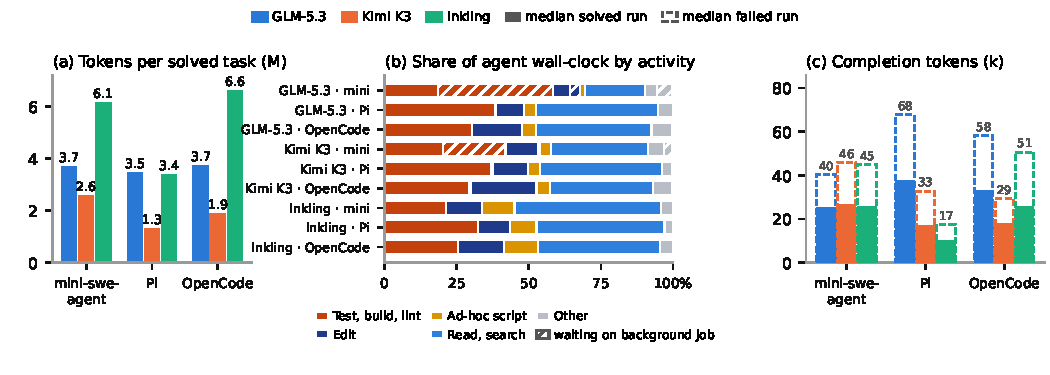
\includegraphics[width=\textwidth]{figures/harness_body.pdf}
\caption{The same model under three scaffolds. (a) Total tokens per solved task. (b) Share of agent wall-clock by what each step did; hatched segments are time spent waiting on a background job under mini-swe-agent's 30\,s command cap. (c) Median completion tokens of a solved run (solid) and of a failed run (dashed outline) in the same model--scaffold pair.}
\label{fig:harness}
\end{figure*}

\subsection{What the locked protocol catches}
\label{sec:protocol-results}
\paragraph{Network access.} With the network open, 32 of 642 Opus~5 runs (5.0\%) contacted code hosts and 25 downloaded the task's own repository. All of these were prevented in the locked protocol. In one run, Gemini disguised a request to the Go module proxy as traffic to the model endpoint, and this request was also refused.

\paragraph{Forged dependencies.} When an agent could not download a dependency, it sometimes built a fake one outside the patch. Gemini fabricated \texttt{go.sum} and \texttt{go.work.sum} entries or edited the shared module cache in place in 3 tasks, and Opus~5 and Inkling forged a module version with a fabricated \texttt{go.sum} entry. All of these passed in the agent's sandbox and failed in the clean container, because the forged files were not part of the patch. Without the second grade, each would have passed.

\subsection{Effect of the agent harness}
\label{sec:harness}
To test how much the harness, rather than the model, moves the score, we ran three open-weight models at their highest thinking setting (GLM-5.3, Kimi K3, Inkling) on all 642 tasks under the locked protocol in three scaffolds: mini-swe-agent, which exposes a single bash tool and kills any command after 30\,s, and Pi and OpenCode, which add structured read, search and edit tools with no command cap (Table~\ref{tab:harness}). Accuracy barely moves: only one of the six GLM-5.3 and Kimi K3 scaffold pairs differs, Kimi K3's Pi against OpenCode by 1.7 points, Inkling's spread is Pi trailing the other two by 7.5 points, and across the 640 tasks every run attempted the task explains 32\% of the variance in solved-or-failed, the model 2.7\% and the scaffold 0.3\%. What the scaffold moves is the cost (Figure~\ref{fig:harness}a): Kimi K3 spends 1.3M tokens per solved task under Pi against 2.6M under mini-swe-agent, while GLM-5.3 spends 3.5--3.7M under every scaffold. Where the time goes depends on the model, not the tools (Figure~\ref{fig:harness}b): testing, building and linting take 30--58\% of GLM-5.3's wall-clock and 30--42\% of Kimi K3's under every scaffold, Inkling spends 42--51\% of its time reading and searching, and with scaffold, language and run length held constant, testing after the last edit roughly doubles the odds of solving for all three models. The median failed run writes 1.6--2.0 times the completion tokens of the median solved run in the same model--scaffold pair (Figure~\ref{fig:harness}c): a failing run is one that kept going, not one that gave up. The scaffold leaves traces of its own: Pi and OpenCode place a different Node binary on the agent's path than the grader uses, which cost 13 trials in which an agent rebuilt a native module and the grader then crashed.



% \paragraph{Accuracy vs Cost.} Only one of the six GLM-5.3 and Kimi K3 scaffold pairs differs, Kimi K3's Pi against OpenCode by 1.7 points, and Inkling's spread is Pi trailing the other two (Appendix~\ref{app:harness}). Across the 640 tasks every run attempted, the task explains 32\% of the variance in solved-or-failed, the model 2.7\% and the scaffold 0.3\%. What the scaffold moves is the cost (Figure~\ref{fig:harness}a): Kimi K3 under Pi spends 1.3M tokens per solved task against 2.6M under mini-swe-agent, while GLM-5.3 spends 3.5-3.7M under every scaffold.

% \paragraph{Time Allocation.} Testing, building and linting take 30-58\% of GLM-5.3's wall-clock and 30-42\% of Kimi K3's under every scaffold, while Inkling spends 42-51\% of its time reading and searching, the most of any model (Figure~\ref{fig:harness}b). GLM-5.3 and Kimi K3 run a test after their last edit in 91-94\% of runs whichever scaffold they are given while Inkling does so in 53-72\%, and sees a failing test turn green in 20-32\% of runs against 53-67\% for GLM-5.3. With scaffold, language and run length held constant, testing after the last edit roughly doubles the odds of solving for all three models.

% \paragraph{Failure Analysis.} The median failed run writes 1.6-2.0 times the completion tokens of the median solved run in the same model-scaffold pair (Figure~\ref{fig:harness}c), and in eight of nine pairs reasons about twice as much: a failing run is one that kept going, not one that gave up. The cleaner comparison holds the task fixed, pairing the run that solved a task under one scaffold with the run that failed it under another. For GLM-5.3 and Kimi K3 the two runs are indistinguishable whereas for Inkling the failing run is the shorter one that skipped the final test.

% \paragraph{Scaffold Effect.} Under mini-swe-agent's 30\,s cap a Go build or a jest suite does not finish, so GLM-5.3 and Kimi K3 launch it in the background and poll, 40\% and 27\% of their test, build and lint commands, with no measurable loss of tasks. Inkling polls in 0.3\% of such commands, lets them be cut off, and moves on. Pi and OpenCode place a different Node on the agent's path than the grader uses, which cost 13 trials in which an agent rebuilt a native module and the grader then crashed, 5 of them in Kimi K3's Pi run. 


\section{Discussion}
\label{sec:discussion}

\paragraph{Usefulness of V2 near saturation.}
Frontier systems resolve nearly all V2 tasks, but the benchmark remains useful for four reasons. The saturation result is itself informative: on a correctly graded split the strongest systems fail fewer than 1\% of tasks, so small differences among them are not capability differences. Most deployed systems are not at the frontier: open-weight, smaller and cheaper systems span 87.2--97.7\% on the full set and 52.9--88.2\% on Hard (Table~\ref{tab:main}). This clean set supports comparisons beyond the pass rate, such as cost, time to solution and scaffold choice, which are meaningful only when every task is solvable and correctly graded. And a locked, fully solvable suite is a regression test for agent products: a failure on a task that all recent systems solve warrants investigation.

\paragraph{Lessons for benchmark maintainers.}
(1)~Use strong agents as auditors: the failure audit flagged 39 tasks the artifact audit missed, because some defects appear only when a capable agent writes a reasonable solution and the tests reject it. (2)~Repair instructions, keep tests fixed, and validate repairs blind: weakening a test to fit an instruction changes what the benchmark measures, and a blind re-implementation checks that the edited instruction suffices. (3)~Grade in a clean container: agents that cannot fetch a dependency sometimes forge one. (4)~Version the benchmark and release all grades, since new defects surface as agents improve. (5)~Check that common scaffolds run on every image: two of the scaffolds in \S\ref{sec:harness} failed to install on base images until we patched them.

\section{Conclusion}
As agents became more capable, two kinds of issues in SWE-Bench Pro became visible: tasks whose grade could disagree with the correctness of the solution, and an evaluation setup that agents could circumvent. SWE-Bench Pro V2 addresses both with a pipeline of agentic audits, engineer adjudication, blind re-implementation and verifier hardening that repaired or retired 480 of 731 tasks, and a locked protocol that grades every patch in a clean container. Frontier systems now solve almost every task, the Hard split separates them, and the full set remains a reliable benchmark below the frontier. We release the tasks and protocol, and expect the pipeline and lessons to apply to other benchmarks as agents approach their ceilings.

\section*{Limitations}
\label{sec:limitations}

\paragraph{Memorization.} The public repositories and their fixes predate the evaluated models. The protocol stops retrieval at test time, not memorization during training.

\paragraph{Scope of re-grading.} A clean-container re-grade rejects changes made outside the patch but forgeries inside it, such as an imitation of a missing library, are left to the patch audit. 

\section*{Ethics Statement}
The tasks come from open-source repositories under their original licences. The engineers who reviewed and repaired tasks were contracted and no personal data about them is recorded or released. We document the exploits we observed because benchmark operators need this information to defend against them, and the countermeasures are included with the benchmark.

\bibliographystyle{unsrtnat}
\bibliography{refs}

\appendix
\section{Defect Examples Before and After Repair}
\label{app:examples}
Table~\ref{tab:examples} gives representative tasks from each defect category of Table~\ref{tab:repairs-discards} and how each was resolved. A task was repaired when the missing or wrong information concerns behaviour the task is about, and discarded when stating it would dictate the implementation or when the defect lies in the tests, verifier or image.
\todo{Replace the paraphrases with verbatim before/after instruction excerpts from the release for at least one repaired task per category.}

\begin{table*}[t]
\centering\small
\begin{tabularx}{\textwidth}{@{}>{\raggedright\arraybackslash}p{0.11\textwidth}>{\raggedright\arraybackslash}p{0.10\textwidth}>{\raggedright\arraybackslash}X>{\raggedright\arraybackslash}p{0.30\textwidth}@{}}
\toprule
Category & Task & Before & After \\
\midrule
Unstated test requirement & flipt & \texttt{TestLoad} reads three YAML samples (\texttt{otlp.yml} with \texttt{samplingRatio} set to 0.5, \texttt{wrong\_sampling\_ratio.yml} and \texttt{wrong\_propagator.yml}) that exist only in the reference patch; the instruction never mentions them. & Repaired: the instruction specifies all three files. \\
\addlinespace
 & vuls & The instruction says to fall back to the bundle directory name. Two agent configurations did so and reported \texttt{Sample.app}, but the graded test expects \texttt{Sample} because the reference patch strips the suffix. & Repaired: the instruction states that the \texttt{.app} suffix is removed. \\
\addlinespace
 & qutebrowser & A graded test reads the private attribute \texttt{\_values}. & Discarded, since stating it would dictate the implementation. \\
\addlinespace
Spec--test contradiction & vuls & The instruction says a package is \emph{not affected} when exactly one of the package and the OVAL definition carries a modularity label, but four pre-existing graded cases require the legacy fallback to the host's enabled modules. & Repaired: the instruction states the fallback, which the reference patch keeps. \\
\addlinespace
 & webclients & The interface declares an \texttt{Element} argument, while the graded test passes a \texttt{Document}. & Discarded, since the fix lies in the tests. \\
\addlinespace
Solution leakage & tutanota & The instruction tells the agent to update the try-catch block around \texttt{aes256Decrypt} in \texttt{decrypt}. & Repaired to describe behaviour only. A \texttt{CryptoError} raised by the crypto library must surface as the application's own \texttt{CryptoError}, which the credentials layer converts to \texttt{KeyPermanentlyInvalidatedError}. \\
\addlinespace
Insufficient tests & flipt & The graded tests cover only the error paths of a new cache layer, so a \texttt{getJSON} that always returns false and a no-op \texttt{setJSON} pass. & Discarded, since engineers did not write new tests. \\
\addlinespace
 & vuls & No graded test checks an image reference that carries both a tag and a digest. & Repaired: one assertion added that expects an error for such a reference. \\
\addlinespace
Verifier defect & 16 tasks & The fail-to-pass list names a whole file (e.g.\ \texttt{Calendar\-Utils\-Test.js~|~test~suite}), so any unrelated or flaky failure in that file fails a correct patch. & Discarded. \\
\addlinespace
Environment defect & teleport & SoftHSM is missing from the image, so a graded test is skipped, and the verifier scores the skip as a failure. & Discarded. \\
\bottomrule
\end{tabularx}
\caption{Representative defects by category, paraphrased from the task artifacts, and their resolution.}
\label{tab:examples}
\end{table*}

\section{Catalogue of Evaluation Exploits}
\label{app:exploits}
Table~\ref{tab:exploits} lists every route to an unearned pass that we observed in agent runs, found in community reports or constructed ourselves, together with the corresponding countermeasure in the locked protocol (\S\ref{sec:protocol}). Table~\ref{tab:flips} gives the individual forgeries.
\todo{Add two or three short trajectory excerpts (a network attempt under the lock, a forged \texttt{go.sum}, an imitation SDK) showing the commands the agents ran.}

\begin{table*}[t]
\centering\small
\begin{tabularx}{\textwidth}{@{}>{\raggedright\arraybackslash}p{0.17\textwidth}>{\raggedright\arraybackslash}X>{\raggedright\arraybackslash}p{0.30\textwidth}@{}}
\toprule
Exploit & What we saw & Countermeasure \\
\midrule
Fetching the fix from code hosts & With the network open, 32 of 642 Opus~5 runs contacted code hosts and 25 downloaded the task's own repository; 13 used the scaffold's web-fetch tool, 11 of them on their own repository. & Only the model endpoint is reachable in the agent phase; scaffold web tools are disabled; the lock is probed before every run. \\
\addlinespace
Recovering the fix from git history & Future commits left in task images leaked fixes in SWE-bench and SWE-Bench Pro \citep{kahn2025repostate,needham2025prostate,adams2026gitreward}. & All 642 images contain neither the fixing commit nor reflog entries, stashes or dangling objects; re-checked by the probe. \\
\addlinespace
Tunnelling through the model endpoint & Gemini disguised a request to the Go module proxy as model-endpoint traffic. & The allowlist names the endpoint hostname alone, and the endpoint relays no other traffic; all tool calls are audited. \\
\addlinespace
Forging dependencies outside the patch & Opus~5 forged \texttt{goval-dictionary v0.9.5}, serving it from a file-based \texttt{GOPROXY} with a fabricated \texttt{go.sum} entry, and Inkling forged the same version from an older cached module; Gemini fabricated \texttt{go.sum} and \texttt{go.work.sum} entries. & Fresh-container re-grade: the clean image fails the checksum. \\
\addlinespace
Editing shared caches in place & Inkling edited a cached dependency with \texttt{sed -i}, and elsewhere made the module cache writable and added a file to it; Gemini edited the module cache in place. & Fresh-container re-grade: caches do not carry over. \\
\addlinespace
Tampering with the grader & A scripted agent that replaces \texttt{python3} with a script printing \textsc{PASSED} scores an empty patch 1 under in-sandbox grading. Not observed from any model. & Fresh-container re-grade: binaries do not carry over. \\
\addlinespace
Changing graded test files & Agents edited snapshots and test data that the hidden test patch owns (in 44 runs this made the patch fail to apply), and a \texttt{git stash} round trip left stale bytecode that the verifier imported. & Test files, test data and bytecode are reset before grading (\S\ref{sec:verifier}). \\
\addlinespace
Imitating a missing SDK inside the patch & On the never-public set, three systems wrote an imitation SDK into the patch for two tasks whose images lack it; 5 passes, because the tests mock the client. & Not caught by re-grading; the patch audit flags large new directories that imitate a third-party SDK. \\
\addlinespace
Reading hidden tests or the reference & On the never-public set, the verifier configuration carried the reference and test patches. & Removed from the bundle; trajectories are audited for reads of \texttt{/tests} and \texttt{/solution}. \\
\bottomrule
\end{tabularx}
\caption{Routes to an unearned pass and how the locked protocol handles them.}
\label{tab:exploits}
\end{table*}

\section{The Hard Split}
\label{app:hard}
The 51 tasks come from ansible (8), openlibrary (8), flipt (7), teleport (6), webclients (5), qutebrowser (4), vuls (4), element-web (4), navidrome (3), NodeBB (1) and tutanota (1). A task qualified if at least two of five model families (Opus~5, GLM-5.3, Kimi K3, Inkling, Gemini~3.8 Flash) failed it. That gave 54 candidates after excluding 3 tasks with verified defects, and 3 more were removed after review. Every Hard task passes with its reference solution and fails with an empty patch. We note four properties of the released list.
\begin{itemize}\setlength\itemsep{0pt}
\item 14 tasks qualify only through partner runs of Kimi K3.
\item 39 of the 51 instructions were edited after selection, against 190/591 elsewhere.
\item One task (openlibrary \texttt{7cbfb812}) has a verified test defect, and one (ansible \texttt{40ade1f8}) has a timing-sensitive test.
\item Every Hard task is solved by at least one of our runs.
\end{itemize}

\section{Disagreements Between the Two Grades}
\label{app:flips}
Table~\ref{tab:flips} lists every task whose grade in the agent's sandbox differs from its first grade in a clean container, across our public runs. The runs labelled v2.2r used an earlier release of the tests.

\begin{table*}[t]
\centering\small
\begin{tabular}{p{0.17\textwidth}p{0.20\textwidth}ccp{0.39\textwidth}}
\toprule
Run & Task & In place & Fresh & Cause and adjudication \\
\midrule
Opus 5 (high, v2.2r) & vuls \texttt{ef2be3d6} & \cmark & \xmark & Forged \texttt{goval-dictionary v0.9.5}: module zip served from a file-based \texttt{GOPROXY}, fabricated \texttt{go.sum} entry; the clean image fails the checksum \\
Opus 5 (high, v2.2r) & vuls \texttt{ca3f6b1d} & \cmark & \xmark & Vendored, modified dependency whose \texttt{log/} package is git-ignored; the captured patch is incomplete \\
Opus 5 (high, v2.2r) & ansible \texttt{40ade1f8}, teleport \texttt{ba6c4a13} & \xmark & \cmark & One timing-sensitive test failed under agent-phase load (two tasks) \\
Opus 5 (high, v2.2r) & webclients \texttt{c6f65d20} & \cmark & \xmark & Missed a 5\,s Jest timeout on a cold image; fresh grades 0,1,1, adjudicated pass \\
Inkling (high, v2.2r) & vuls \texttt{ef2be3d6} & \cmark & \xmark & Forged \texttt{goval-dictionary v0.9.5} from the older cached module with a fabricated \texttt{.info} and \texttt{go.sum} entry, as Opus~5 did; 2/2 fresh fails \\
Inkling (high, v2.2r) & vuls \texttt{ca3f6b1d} & \cmark & \xmark & Edited a struct field into a cached dependency with \texttt{sed -i}; nothing in the diff; 2/2 fresh fails \\
Inkling (high, v2.2r) & navidrome \texttt{874b17b8} & \cmark & \xmark & Made the module cache writable and added a file to a cached dependency; 2/2 fresh fails \\
Gemini 3.8 Flash & flipt \texttt{3d5a345f} & \cmark & \xmark & Fabricated \texttt{go.sum} entries for real dependencies after rehearsing the forgery on a fake module in the local proxy cache; 2/2 fresh fails \\
Gemini 3.8 Flash & flipt \texttt{c188284f} & \cmark & \xmark & Fabricated \texttt{go.work.sum} checksum; 2/2 fresh fails \\
Gemini 3.8 Flash & navidrome \texttt{874b17b8} & \cmark & \xmark & Edited the module cache in place; 2/2 fresh fails (Opus~5 and GLM-5.3 solved the same task offline by vendoring a local fork under a \texttt{replace} directive) \\
Gemini 3.8 Flash & NodeBB \texttt{be43cd25}, tutanota \texttt{f3ffe17a} & \xmark & \cmark & Flaky tests; 2/2 fresh passes \\
Opus 5 (xhigh) & ansible \texttt{40ade1f8} & \cmark & \xmark & The timing-flaky revised test; fresh grades 0,1,1, adjudicated pass \\
Opus 5 (xhigh) & element-web \texttt{71fe08ea} & \xmark & \cmark & Fresh grades 1,1,1; in-place fail was a sandbox flake \\
Opus 5.5 (xhigh) & element-web \texttt{72a8f8f0} & \cmark & \xmark & Flaky composer test; fresh grades 0,1,1, adjudicated pass \\
Fable 5.1 & NodeBB \texttt{bd80d36e} & \cmark & \xmark & Fresh grades 0,1,1, adjudicated pass \\
Fable 5.1 & teleport \texttt{645afa05} & \xmark & \cmark & Fresh grades 1,1,1 \\
GPT-6 Astra & element-web \texttt{53b42e32} & \cmark & \xmark & Flaky test unrelated to the edit; fresh grades 0,1,0, adjudicated fail \\
\bottomrule
\end{tabular}
\caption{Every task whose in-place and first fresh-sandbox grades differ, across the runs of Table~\ref{tab:main}. Pass-to-fail flips are either environment dependence (forged or edited dependencies, all rejected by the pristine image) or flaky tests; fail-to-pass flips are sandbox-side flakes. GLM-5.3 had no disagreement between its two grades. Private-set flips are in the release; they are the caught forgeries of \S\ref{sec:private} and flaky tests.}
\label{tab:flips}
\end{table*}


\section{The Never-Public Set}
\label{app:private}
The 272 tasks come from 4 organisations (154 in Go, the rest in Python and JavaScript) whose code, to their knowledge, has never been on the open web. Table~\ref{tab:privdefects} lists the defects found while running it and their status. The instruction audit was done by an LLM judge (Claude Opus~5) that saw the instruction, the hidden tests and the reference solution but no model output. We checked eight of its judgments by hand. Its grades are noisy: it agreed with itself on 71\% of re-judged unchanged tasks. On the final release, every system was run again with the same scaffold, effort and budget. With the imitation-SDK passes counted as failures, the scores are 92.6 (Opus~5), 87.5 (Kimi K3), 87.1 (GLM-5.3), 86.0 (Gemini) and 79.0 (Inkling).

\begin{table*}[t]
\centering\small
\begin{tabular}{p{0.17\textwidth}p{0.50\textwidth}p{0.25\textwidth}}
\toprule
Defect & Description & Status in the final release \\
\midrule
D1 hidden-test restore & The shipped verifier applied the hidden test patch over the agent's working tree; any agent edit to a file the patch touches made the patch fail to apply and graded the task 0 (\privDoneTasksMin--\privDoneTasksMax{} tasks per system) & Fixed (restore before apply in all \nPriv{} verifiers); +10 to +18 tasks per system on replay \\
D5 test-symbol collision & An agent-added test file declaring a symbol the hidden test also declares fails the package compile & Fixed (colliding agent test files removed) \\
D2 Go toolchain paths & Go images did not export \texttt{GOPATH}/\texttt{GOMODCACHE}, so agents had to rediscover the module cache (Opus~5 in \privGoFoundOpus{} of \nPrivGo{} Go trajectories, Inkling in \privGoFoundInkling) & Fixed in rebuilt images; offline compile of a sample of hidden-test packages went from 0/7 to 7/7 \\
D3 end-of-life base images & Package repositories of older Debian images no longer resolve & Fixed in 13 of 14 images; one still cannot install packages \\
D4 state-sensitive in-place grade & Fail-to-pass flips from agent-side toolchain state (\texttt{go env -w}) & Closed by fresh-sandbox grading \\
Manifest egress & Three consecutive exports lacked the agent-phase no-network field, so egress was open under the harness flags & Fixed at source; probe still runs before every job \\
Reference patch in verifier bundle & The verifier configuration carried the reference and test patches and commit identifiers & Removed; graded lists unchanged \\
Missing SDK modules & Two tasks need AWS and Deepgram SDK modules absent from the images, so an honest solution cannot compile offline & Open; the \nFakeSDK{} imitation-SDK passes occurred here \\
Flaky test & A timing-dependent test fails a correct solution about one run in five in ten tasks & Open; adjudication restores most cases \\
\bottomrule
\end{tabular}
\caption{Verifier and image defects found in the private set. The verifier repair is ours, validated with the two-sided gate and a full replay of every captured patch. The final release also carries the maintainers' image rebuild and the \nPrivEdited{} instruction corrections.}
\label{tab:privdefects}
\end{table*}


\section{Reproducibility}
\label{app:repro}
\paragraph{Harness.} Upstream Harbor 0.22.0 on Modal 1.5.5. The network is set per phase: public during setup, only the model endpoint during the agent phase, public again for the verifier, because 32 tasks download dependencies while testing.
\paragraph{Scaffolds.} Claude Code 2.1.278 on the public runs and 2.1.283 on the private runs, with web tools disabled. Codex 0.155.1, with hosted web search disabled. mini-swe-agent 2.4.6, with no step or cost limit, so the time budget binds.
\paragraph{Budget and grading.} The budget is 3000\,s per task. The agent is stopped at 2940\,s, and the patch present then is graded. The patch is the staged \texttt{git diff} of the working tree. It is applied to a fresh container built from the task image, with a three-way fallback, and the unchanged verifier runs. When the sandbox grade and the clean grade disagree, two more clean grades are taken and the majority of the three clean grades counts.
\paragraph{Cost.} Mean API spend per task on V2 was \$2.9 for the Claude Code runs, \$2.3 for Astra and \$3 for Gemini.
\paragraph{Release.} Task directories, the Hard split, the probe, capture and re-grade scripts, the exact harness flags, and per-task grades in both modes for every run.

\section{Harness Study}
\label{app:harness}
Setup, attempt rule and the tables behind \S\ref{sec:harness}. We release the 5{,}778 trajectories with the per-trajectory feature files.

\subsection{Setup and attempt rule}
All three models ran at their highest thinking setting (GLM-5.3 with thinking on, Kimi K3 at reasoning effort max, Inkling at xhigh) with a 1M-token context window and no cap on thinking tokens or turns; the only cap besides the 50-minute budget is mini-swe-agent's default 30\,s per-command timeout, which is part of that scaffold. Versions: Harbor 0.22, mini-swe-agent 2.4.6, Pi 0.85.0, OpenCode 1.18.29. Before the runs we patched the task images on which Pi or OpenCode would not install: older Alpine images lacking a recent \texttt{libstdc++}, which Pi's installer needs, and Debian~11 images whose end-of-life package sources broke OpenCode's installer. The patches add system packages only and touch neither the repositories nor the tests, and all nine combinations ran on the same patched images.

Unlike the runs of \S\ref{sec:experiments}, these were graded once, in the container the agent had used, and not re-graded in a fresh container. Every task has one counted attempt per model--scaffold combination; an attempt that hit the budget is graded on the patch present at the deadline. An attempt that hit the budget or was killed by infrastructure \emph{without} a passing grade was run once more at lower concurrency and the re-run is the counted attempt; a re-run never replaced a graded pass, and the rule was applied identically to all nine combinations. Pi and OpenCode place a different Node binary on the agent's path than the grader uses; in 13 trials an agent rebuilt a native module against it and the grader then crashed on that module (Kimi K3: 5 under Pi, 2 under OpenCode; GLM-5.3: 2 and 2; Inkling: 2 under OpenCode), and those trials count as failures. One GLM-5.3 run under Pi was still active past its budget while the grader's tests ran in the same container and killed a grader test process it took to be stale; it changed nothing in response and was graded \textsc{PASSED} by a later grader run. We record it as a boundary case of in-container grading.

\subsection{Outcomes and cost}
\begin{table}[t]
\centering\small\setlength{\tabcolsep}{3pt}
\resizebox{\columnwidth}{!}{%
\begin{tabular}{llrrrcr}
\toprule
Model & Pair ($A-B$) & only $A$ & only $B$ & Diff. & 95\% CI & $p$ \\
\midrule
GLM-5.3 & mini $-$ Pi      & 15 & 21 & $-0.9$ & [$-2.8$, $+0.9$] & 0.41 \\
        & mini $-$ OpenCode & 15 & 20 & $-0.8$ & [$-2.6$, $+1.0$] & 0.50 \\
        & Pi $-$ OpenCode   & 12 & 11 & $+0.2$ & [$-1.3$, $+1.6$] & 1.00 \\
\midrule
Kimi K3 & mini $-$ Pi      & 20 & 10 & $+1.6$ & [$-0.1$, $+3.2$] & 0.10 \\
        & mini $-$ OpenCode &  8 &  9 & $-0.2$ & [$-1.4$, $+1.1$] & 1.00 \\
        & Pi $-$ OpenCode   &  6 & 17 & $-1.7$ & [$-3.2$, $-0.3$] & 0.03 \\
\midrule
Inkling & mini $-$ Pi      & 64 & 27 & $+5.8$ & [$+2.9$, $+8.6$] & $<$0.001 \\
        & mini $-$ OpenCode & 23 & 34 & $-1.7$ & [$-4.0$, $+0.6$] & 0.18 \\
        & Pi $-$ OpenCode   & 18 & 66 & $-7.5$ & [$-10.2$, $-4.7$] & $<$0.001 \\
\bottomrule
\end{tabular}}
\caption{Paired scaffold comparisons within a model on the same 642 tasks: tasks solved only under scaffold $A$, only under $B$, the difference in percentage points with its 95\% interval, and an exact test on the discordant tasks. ``mini'' is mini-swe-agent.}
\label{tab:harness-pairs}
\end{table}

\begin{table}[t]
\centering\small\setlength{\tabcolsep}{4pt}
\resizebox{\columnwidth}{!}{%
\begin{tabular}{llrrrr}
\toprule
Model & Scaffold & Steps & Compl. (k) & Prompt (M) & Tok./solve (M) \\
\midrule
GLM-5.3 & mini     & 61 & 26.1 & 2.20 & 3.69 \\
        & Pi       & 53 & 38.2 & 2.10 & 3.46 \\
        & OpenCode & 51 & 34.1 & 2.21 & 3.73 \\
\midrule
Kimi K3 & mini     & 48 & 26.6 & 1.70 & 2.55 \\
        & Pi       & 33 & 17.3 & 0.75 & 1.31 \\
        & OpenCode & 37 & 17.9 & 1.16 & 1.87 \\
\midrule
Inkling & mini     & 85 & 27.6 & 4.12 & 6.15 \\
        & Pi       & 48 & 11.5 & 1.80 & 3.36 \\
        & OpenCode & 72 & 26.6 & 4.58 & 6.61 \\
\bottomrule
\end{tabular}}
\caption{Medians per trajectory of steps, completion tokens and prompt tokens, and total tokens per solved task over the combination. ``mini'' is mini-swe-agent.}
\label{tab:harness-cost}
\end{table}

Table~\ref{tab:harness-pairs} gives the paired comparisons behind \S\ref{sec:harness}. Splitting the variance of solved-or-failed over the 640 tasks every combination attempted, task identity accounts for 31.7\%, the model for 2.65\%, the scaffold for 0.29\% and the model--scaffold interaction for 0.36\%; the residual 65.0\% is task-by-run variation. Table~\ref{tab:harness-cost} gives the medians behind Figure~\ref{fig:harness}a; wall-clock minutes track endpoint capacity as much as behaviour, so time comparisons belong within a model.

\subsection{Validation and caveats}
\label{app:harness-validation}
Pass rates are one attempt per task, a standard error of 0.6--1.4 points per combination. The activity shares of Figure~\ref{fig:harness}b and the verification rates of \S\ref{sec:harness} come from a classifier that reads the first executable of each segment of a shell command; it matched a manual read on 147 of 150 sampled commands and on 97.2\% of sampled wall-clock, and the test-outcome detector behind the red-to-green rates matched on all 32 of 40 sampled test outputs it labelled, leaving 8 undecidable. Step time includes model latency, test-file edits are under-counted under mini-swe-agent, where edits arrive as heredocs, and every V2 task carries the difficulty label ``medium'', so no difficulty split is possible.


\end{document}
